\begin{figure}
    \begin{fullwidth}
    \centering
    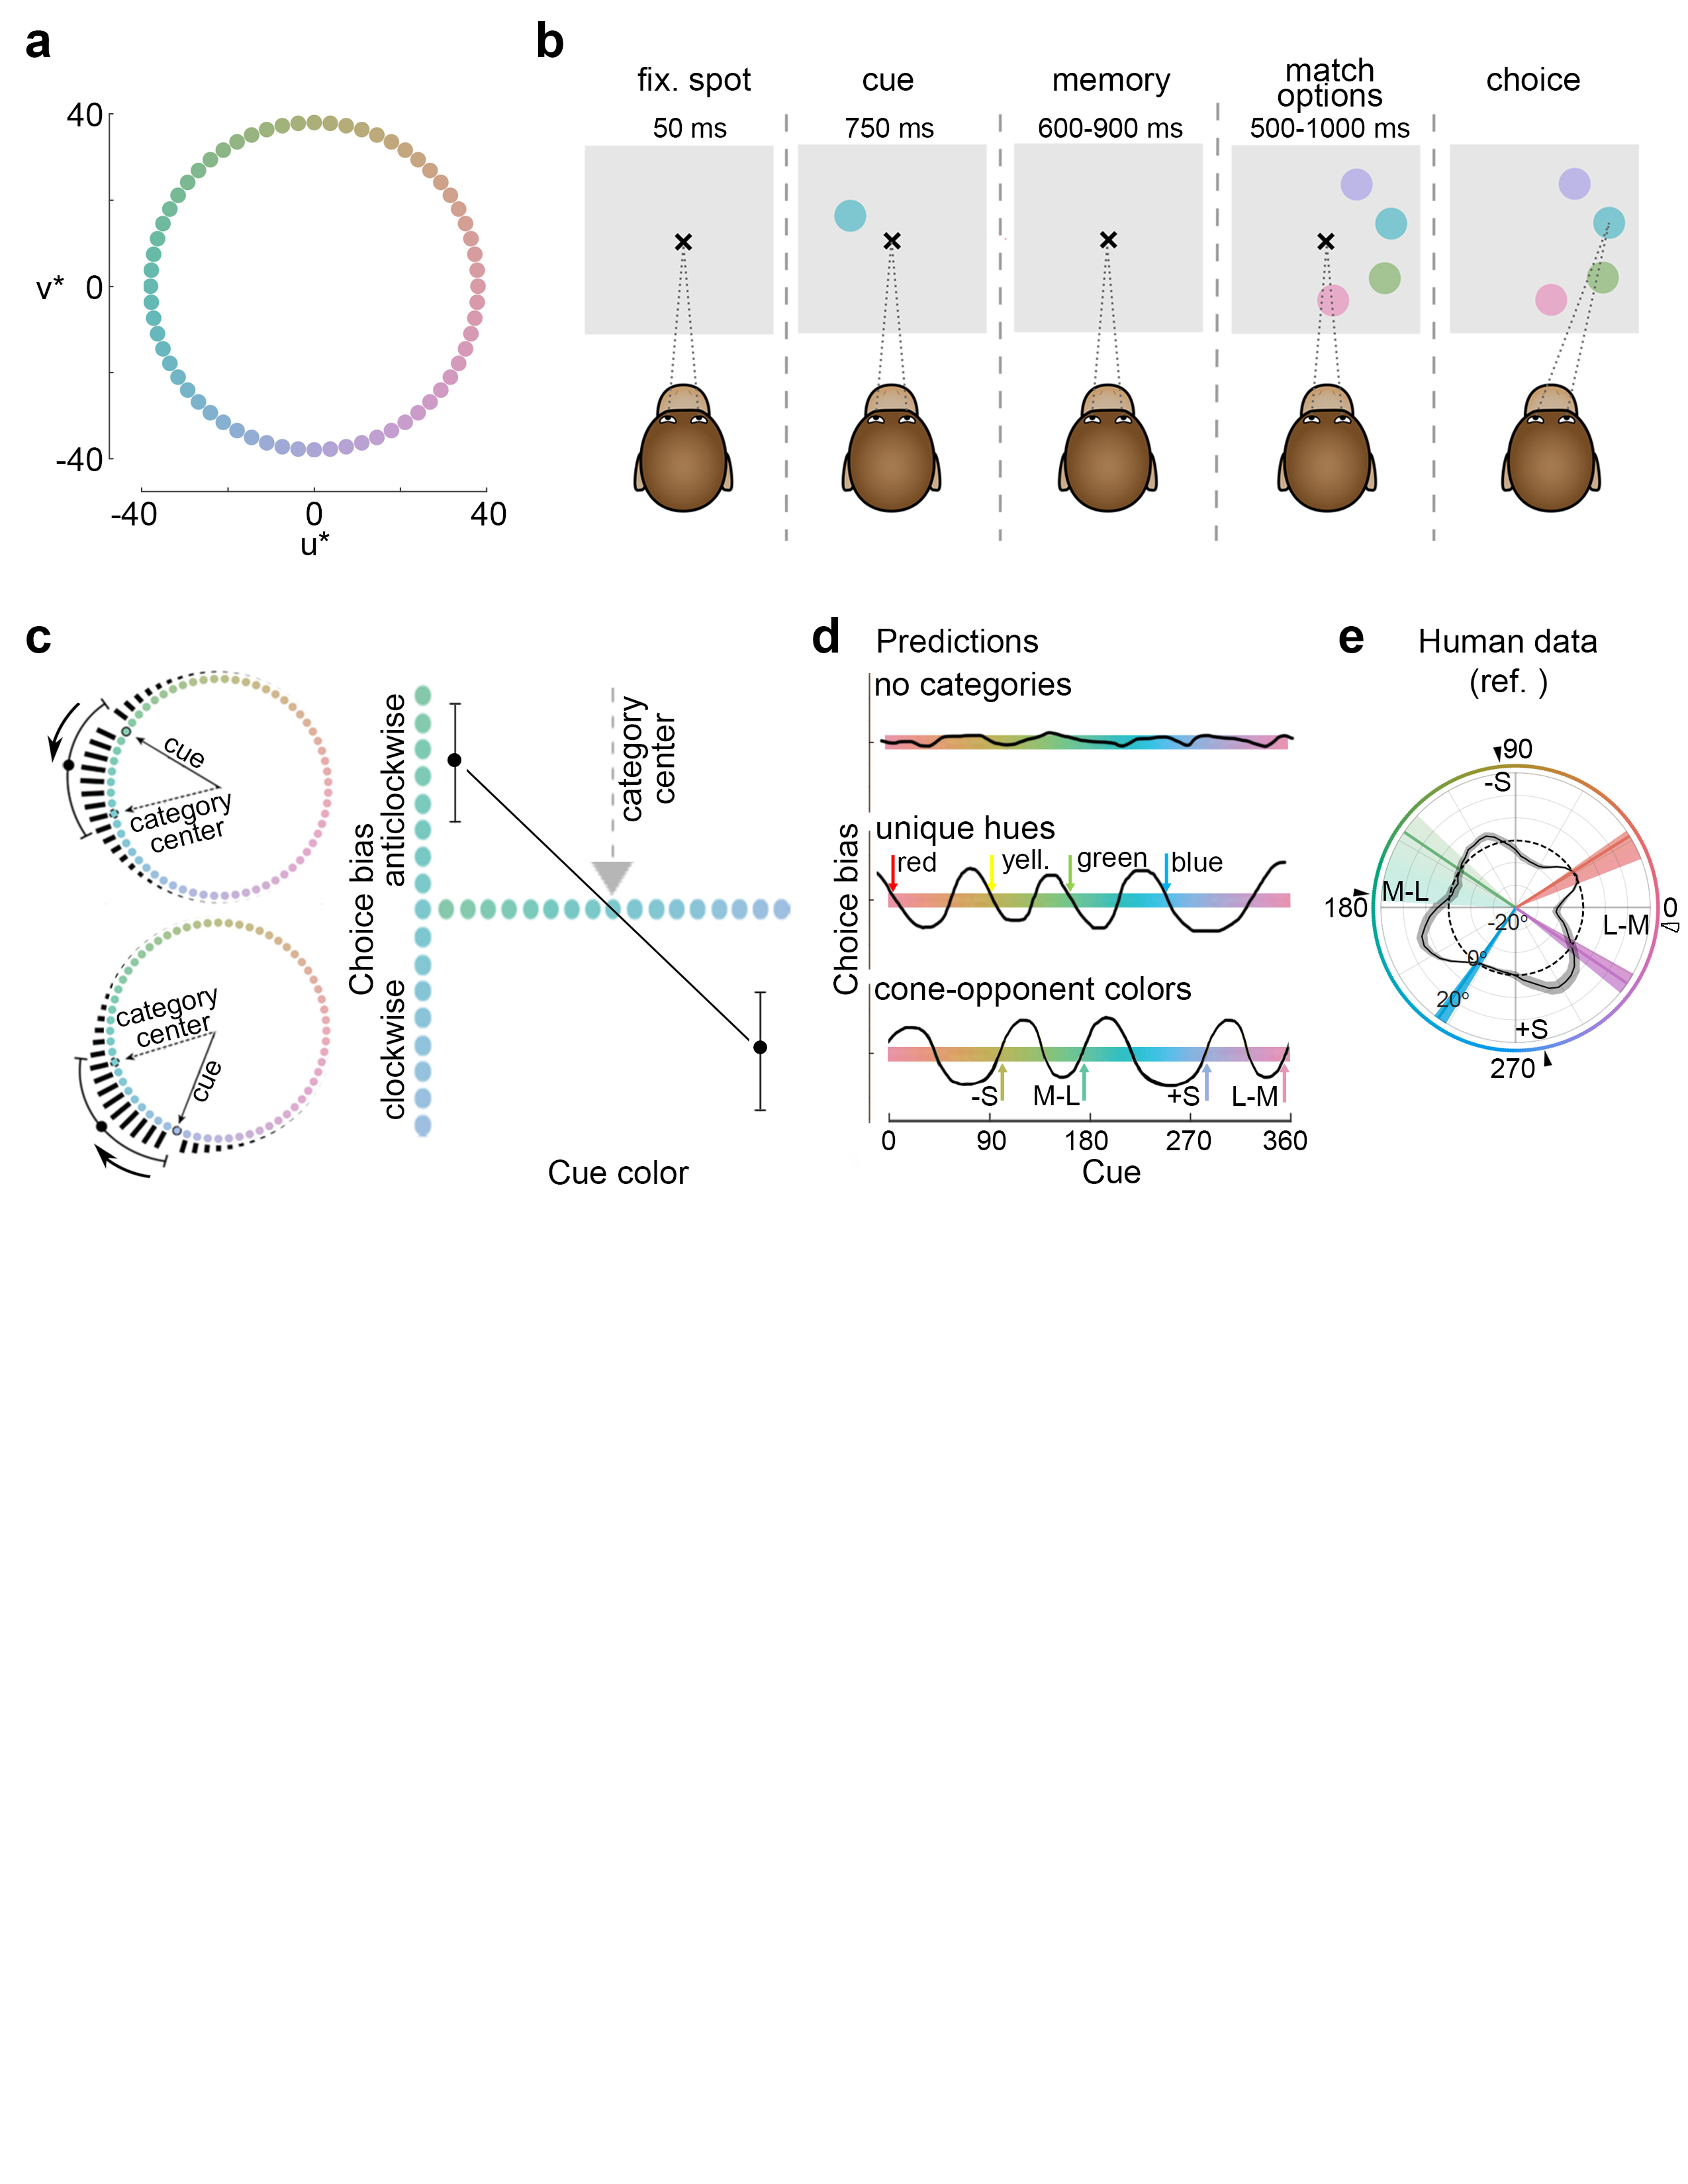
\includegraphics[width=\textwidth+4cm,trim={0 12.5cm 0 0},clip]{../Figures/flat/F1_ParadigmPredictions_6.jpg}
    \caption{\textbf{Non-verbal paradigm to recover color categories in non-human primates.}
    \textbf{a}, Colors defined in CIELUV color space. 
	\textbf{b}, Animals were trained to initiate a trial by fixating a small cross on a computer monitor and to maintain fixation throughout the trial until the fixation cross disappeared, which was their instruction to make a choice; trials in which the animals broke fixation were aborted. 
	A 3-degree diameter cue was presented within the central 2.5 – 6-degrees, followed by a variable memory delay (600-900ms) and the presentation of the choice options. 
	To mitigate impulsive choices, the choice options were shown for a variable amount of time (500-1000 ms) during which the animals needed to maintain fixation to avoid aborting the trial. After the fixation cross disappeared, the animals were free to make their selection. 
	\textbf{c}, Predicted distribution of choices for two cues if a color category exists at the specified location in the color space (dashed arrow). 
	The average of the distribution of choices will be shifted counterclockwise from the cue if the cue is displaced clockwise to the category center (top) and shifted clockwise from the cue if the cue is displaced counterclockwise to the category center (bottom). This pattern of results would be captured as the zero-crossing of the negative slope in a plot of the choice bias versus cue color (right). 
	\textbf{d}, Predicted pattern of results for three hypotheses: no categories (top); the four most prominent basic color categories (also called the unique hues, middle); and the colors corresponding to the cone-opponent retinal encoding mechanisms (bottom). 
	\textbf{e}, Data obtained in prior work on a related task in human subjects (see SI Figure 1) for three other data sets in human subjects, showing consistent pattern of results). 
    Category centers seem to exist for colors that would be labeled in English as orange, green, blue, and purple. 
	In the polar plot, the negative slopes demarking category centers are recovered by tracing the line in a counterclockwise direction, at points where it crosses the dashed circle marking zero choice bias.
    Repeller points (zero crossings of positive slope) appear to align with the -S, +S, and M-L poles of the cone-opponent axes (solid arrowheads), but not the L-M pole (open arrowhead).} 
    \label{fig:ParadigmAnalysisPredictions}
    \end{fullwidth}
\end{figure}

Color categories are identified by color terms, of which the Basic Color Terms are considered prominent \citep{berlin_basic_1969}.
One hypothesis is that some subset of these terms are universal \citep{heider_universals_1972,regier_focal_2005}
and endowed by hard-wired neural mechanisms present at birth \citep{bornstein_categories_1976,lindsey_universality_2006}. 
This idea, put forth 150 years ago \citep{hering_zur_1875}, predicts some of the consistencies observed in color naming patterns across cultures \citep{jameson_evolutionary_2009,baronchelli_modeling_2010,lindsey_hunter-gatherer_2015,abbott_focal_2016}
and is consistent with some neurophysiological results \citep{clifford_electrophysiological_2009,holmes_neurophysiological_2009,brouwer_categorical_2013,bird_categorical_2014,yang_cortical_2016,forder_colour_2017}. 
Behavioral work in infants provides evidence for a biological origin of color categories \citep{franklin_new_2004,ozturk_language_2013}, but suggests that the innate categories are defined by retinal cone-opponent mechanisms rather than basic colors \citep{skelton_biological_2017,maule_color_2019}.
The infants in these experiments are typically several months old, by which stage they have had substantial cultural exposure, so evidence for color categories cannot conclusively be ascribed an innate origin.
Another hypothesis is that color categories emerge in development, instructed by language and culture \citep{roberson_color_2005, regier_language_2009, cibelli_sapir-whorf_2016}, and possibly involving an interplay of innate and developmental factors \citep{kay_language_2006,franklin_lateralization_2008,regier_language_2009}. 
This hypothesis is promoted by variability in color naming patterns across languages and individuals \citep{davidoff_colour_1999,roberson_color_2000,paramei_online_2018,webster_variations_2002}.
Current consensus is that some aspect of adult color category behavior is acquired through experience; the extent to which color categories are innate remains unresolved \citep{davidoff_nature_2009,skelton_colour_2023}.

An alternative approach to the origin of color categories could be provided by studying trichromatic non-human primates \citep{siuda-krzywicka_biological_2019}. 
The few studies on this topic have come to different conclusions: one found color categories in macaque monkeys seemingly consistent with categories in human adults \citep{sandell_color_1979}. 
This study inadvertently made comparisons substantially easier for cross-category than within-category trials, undermining its conclusion \citep{davidoff_cross-species_2010}. 
A later study tested for the existence of color categories across a limited range of colors and found a blue-green boundary in humans but not baboons \citep{fagot_cross-species_2006}.
The lack of color categories in the non-human primates could simply reflect the limited survey of color space. 
A third study, designed to investigate visual working memory, had two animals match color samples to a continuous ring of colors \citep{panichello_error-correcting_2019}. 
The experimental design is useful for studying visual working memory but complicates interpretation regarding color categorization because the animals could have been rewarded for making inaccurate matches, which would reinforce idiosyncratic biases, and indeed the two animals showed different patterns of behavior.

\paragraph{Measuring color categories in macaque monkeys}

Addressing the question of color categories in monkeys requires overcoming several challenges. 
First, how to measure color categories without teaching the animals the categories or reinforcing idiosyncratic biases \citep{essock_color_1977,matsuno_color_2004}.
Second, how to specify the color stimuli \citep{siuda-krzywicka_biological_2019}; for example, specifying the colors as wavelengths \citep{sandell_color_1979}
is not appropriate \citep{davidoff_cross-species_2010}. 
Third, how to obtain precise data across the full circle of hues so as to avoid missing categories \citep{fagot_cross-species_2006}.
A match-to-sample paradigm using colors defined in a perceptually uniform color space (Figure 1a) provides a potential solution to these challenges, because color categories would be expected to introduce biases in the distribution of matches, so one could infer a color category from measured biases \citep{bae_why_2015}.  
In the standard paradigm, a person is shown a color and asked to match the color to a continuous ring of colors, which is satisfactory for use in human participants who can follow instructions but introduces complications for use in monkeys.
We adapted the paradigm as an alternative-forced-choice task in which a direct match to the cue was available in every trial and the monkeys were only rewarded for making the direct match (Figure 1b). 
This task ensures precision in the matched colors and avoids the possibility of reinforcing biases acquired while the animals perform the task.
One consequence of this adapted paradigm is that it requires considerable data to sample category performance across the space of colors. 
Four animals performed the task, completing a total of 209456 trials over 232 sessions (see SI Figure 2).

If a monkey has a color category, the category center will be an attractor in the color space, captured by a zero-crossing of negative slope in a plot of the choice bias (Figure 1c). 
Repellor points would be captured by the zero-crossing of the positive slope.
The approach is data-driven so it will recover whatever categories exist; nonetheless, before collecting the data we considered three possibilities. 
First, that the monkeys would show no color categories, as predicted by the work sampling a limited range of colors in baboons \citep{davidoff_cross-species_2010}
(Figure 1d, top);
second, that macaque color categories would correspond to  four main basic color categories as predicted by data in human adults (Figure 1d, middle); 
and third, that macaque color categories would align with repellants marked by the cone-opponent mechanisms as predicted by data in human infants \citep{skelton_biological_2017} (Figure 1d, bottom). 
Results in human participants, across multiple variants of the color-matching task in studies from different groups, clearly show evidence for four categories \citep{bae_why_2015,panichello_error-correcting_2019}, matching the number of categories stipulated in the second and third hypotheses but not clearly distinguishing them (Figure 1e; SI Figure 1) — the categories correspond to green, blue, orange, and pink. 

One possibility raised by the prior literature is that these differ from the canonical set of four basic colors (green, blue, yellow, red) because of limitations imposed by ensuring equal saturation and luminance among the colors (see \citep{bae_why_2015}). 
